%%% lorem.tex --- 
%% 
%% Filename: lorem.tex
%% Description: 
%% Author: Ola Leifler
%% Maintainer: 
%% Created: Wed Nov 10 09:59:23 2010 (CET)
%% Version: $Id$
%% Version: 
%% Last-Updated: Wed Nov 10 09:59:47 2010 (CET)
%%           By: Ola Leifler
%%     Update #: 2
%% URL: 
%% Keywords: 
%% Compatibility: 
%% 
%%%%%%%%%%%%%%%%%%%%%%%%%%%%%%%%%%%%%%%%%%%%%%%%%%%%%%%%%%%%%%%%%%%%%%
%% 
%%% Commentary: 
%% 
%% 
%% 
%%%%%%%%%%%%%%%%%%%%%%%%%%%%%%%%%%%%%%%%%%%%%%%%%%%%%%%%%%%%%%%%%%%%%%
%% 
%%% Change log:
%% 
%% 
%% RCS $Log$
%%%%%%%%%%%%%%%%%%%%%%%%%%%%%%%%%%%%%%%%%%%%%%%%%%%%%%%%%%%%%%%%%%%%%%
%% 
%%% Code:

\chapter{Method} \label{cha:method}

    \begin{figure}[h]
        \centering
        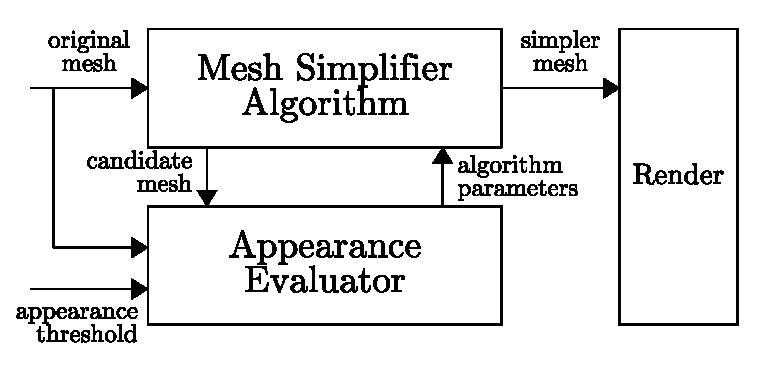
\includegraphics[width=0.7\textwidth]{figures/system_overview.eps}
        \caption{System overview}
        \label{fig:system_overview}
    \end{figure}

    \section{Implementation} \label{sec:implementation}
    Before any mesh simplification algorithm can be integrated into Configura's CET Designer they need to be evaluated. Therefore, an appearance evaluator is implemented first taking the original mesh and a simplified version.

    One possibility is to implement the algorithms and the evaluator directly in Configura's language CM. However, we first only want to evaluate the algorithms wihtout overhead that may be introduced by CET Designer. Therefore, we decided to implement and evaluate them outside CET Designer with a simple renderer based on \emph{OpenGL}.

    To be able to change between the different algorithms, a common interface is implemented that can interact with the appearance evaluator. As seen in figure~\ref{fig:system_overview} the simplification algorithm takes a mesh and then gives a simplified mesh to the evaluator which will compare it to the original mesh. The simplification will be performed until a given appearance-threshold is reached.

    A quick overview of how the algorithms work is explained in the theory chapter. But a more detailed description of how they are implemented for the purpose of the evaluation will be described in the following sections. However, these sections will be left empty at the moment since the implementations is not done for the scientific method course.

        \subsection{Quadric-Based Error Metric} \label{sub:quadric-based_error_metric}

        \subsection{Appearance-Preserving Simplification} \label{sub:appearance-preserving_simplification}

        \subsection{Texture Mapped Progressive Meshing} \label{sub:texture_mapped_progressive_meshing}

    \newpage

    \section{Evaluation} \label{sec:evaluation}

        In order to determine which of these algorithms provide the best performance for a target appearance threshold, an evaluation of the polygon count, computation time, memory usage and rendering time of the simplified mesh is done for each of the implemented solutions. In the results from this step, a series of tables are generated to compare the performance between the algorithms by using a common comparison framework. In this section, we describe this common comparison framework and then show how we can measure each of the parameters.

        In essence, this is done by targeting a certain appearance threshold, tweaking the mesh simplification algorithm's parameters to achieve this threshold, and then measuring the given performance. This gives a universal measure of ``quality'' for all of the algorithms, which would otherwise have different error metrics used for applying the simplification. Since the performance measures are noisy, a total of \(n=20\) samples will be taken. According to \emph{David Lilja}~\cite[p.~50]{lilja2005measuring} the t-student distribution should be used when \(n < 30\), as shown in Section~\ref{sec:measuring_algorithmic_performance}.

        The pack of test meshes that are going to be used in the comparison are a combination of textured models provided by Configura and others taken from the public domain. The exact selection of these is still to be decided, but should include both low- \& high-polygon meshes.

        \subsection{Appearance Preservation} \label{sec:appearance_preservation}
        In order to compare the appearance preservation of the mesh simplification algorithms, the image-metric explained in section~\ref{sec:metrics_for_appearance_preservation} is used. It is useful since it can compare the difference of any two meshes, therefore, it does not depend on the algorithm used.

        For both the original mesh and a simplified mesh, 24 images with resolution $512 \times 512$ is rendered with a simple renderer based on \emph{OpenGL}. The camera is placed at the vertices of a rhombicuboctahedron and is faced towards the center where the mesh is placed. A light source is placed at the camera position. This will make sure that the surface facing the camera will be illuminated.

        The two sets of 24 images each is used to compute the RMS of the simplified mesh with equation~\ref{eq:rms_image_sets}. This RMS value can then be used to compare how well the algorithms perform. 
        \subsection{Polygon Count} \label{sec:polygon_count}
        Concerning research question 3, the appearance preservation for a specific target polygon count needs to be measured. Therefore, the simplification algorithms is tasked to simplify until the target polygon count is reached. When it is reached, the image-metric is used to measure how well the appearance is preserved. Measurements will be performed for multiple target polygon counts. 

        \subsection{Computation Time} \label{sec:computation_time}

        An important property of a mesh simplification algorithm is the time it takes to simplify a full-resolution mesh to a lower-resolution mesh. While this doesn't impact the run-time of the mesh (that is accounted for by the rendering time, measured in Section~\ref{sec:rendering_time}), it is still important to reduce it as much as possible. This is especially true if the LoD is dynamically generated at run-time, but it is also important since many more meshes can be simplified per time unit (important if a simplifier is to be provided as a service, as \emph{Simplygon Linköping} does).

        In order to compare the execution time of the different algorithms, they all target the same appearance thresholds as specified in Section~\ref{sec:appearance_preservation} by tweaking the parameters unique to each algorithm. We then measure the time it takes for the simplification algorithm to execute when using these parameters, in other words, simply by: \(time_\mathcal{A} = end_\mathcal{A} - start_\mathcal{A}\) for an algorithm \(\mathcal{A}\). Of course, this measurement is done several times to account for noise. After calculating the mean \(\bar{x}\) and the standard-deviation \(s\), one can find the confidence interval \([a, b]\) of the execution time by the equations shown in Section~\ref{sec:measuring_algorithmic_performance} with 19 degrees of freedom and \(\alpha = 5 \%\).

        \subsection{Memory Usage} \label{sec:memory_usage}

        Another important performance property of the algorithm is the accumulated memory used when simplifying the mesh. Depending on the size of the mesh in triangles, the algorithm could consume large amounts of memory (and might not even fit in the primary memory in some cases). It is therefore important to compare the simplification algorithms to determine those which are suited for optimizing large triangle meshes and those that aren't. Since this measure will always be deterministic (at least for the method we use to measure it), there is no need to apply any statistical measures. The \emph{Valgrind} suite was chosen since it has the \emph{Massif} heap profiler, which gives accurate memory usage. According to the \emph{Massif documentation}~\cite{valgrind2017manual} there is an expected slowdown of 20x, which isn't a problem since the computation time and rendering time are measured separately. Below are the commands to find the memory usage.

        \begin{lstlisting}[language=bash]
 (*\textbf{valgrind}*) --tool=massif (*\textit{./simplify --algorithm=<algorithm> <input-mesh> <output-mesh>}*)
        \end{lstlisting}

        \subsection{Rendering Time} \label{sec:rendering_time}
        One main purpose of simplifying a mesh is to reduce the rendering time. Therefore, the frame rate is measured when rendering the original mesh and the simplified meshes. The simplified meshes comes from the previous steps where different appearance-thresholds was targeted. Frame rate is measured by counting how many frames that have been rendered during a period of one second. As with computation time, this measurement may have noise and therefore multiple samples needs to be obtained. The mean and condifidence interval is obtained in the same way.

%%%%%%%%%%%%%%%%%%%%%%%%%%%%%%%%%%%%%%%%%%%%%%%%%%%%%%%%%%%%%%%%%%%%%%
%%% method.tex ends here

%%% Local Variables: 
%%% mode: latex
%%% TeX-master: "thesis"
%%% End: 
